\documentclass[10pt]{article}

\usepackage[applemac]{inputenc}
\usepackage[english]{babel}
\usepackage[T1]{fontenc}
\usepackage{cite, url,color} % Citation numbers being automatically sorted and properly "compressed/ranged".
%\usepackage{pgfplots}
\usepackage{graphics,amsfonts}
\usepackage[pdftex]{graphicx}
\usepackage[cmex10]{amsmath}
% Also, note that the amsmath package sets \interdisplaylinepenalty to 10000
% thus preventing page breaks from occurring within multiline equations. Use:
 \interdisplaylinepenalty=2500
% after loading amsmath to restore such page breaks as IEEEtran.cls normally does.

%% Useful packages for creation of two-column and more complex figures
% Compact lists
\usepackage{enumitem}
\usepackage{booktabs}
\usepackage{fancyvrb}

\usepackage{listings} % inserisce listati di programmi
\definecolor{commenti}{rgb}{0.13,0.55,0.13}
\definecolor{stringhe}{rgb}{0.63,0.125,0.94}
\lstloadlanguages{Matlab}
\lstset{% general command to set parameter(s)
framexleftmargin=0mm,
frame=single,
keywordstyle = \color{blue},% blue keywords
identifierstyle =, % nothing happens
commentstyle = \color{commenti}, % comments
stringstyle = \ttfamily \color{stringhe}, % typewriter type for strings
showstringspaces = false, % no special string spaces
emph = {for, if, then, else, end},
emphstyle = \color{blue},
firstnumber = 1, % numero della prima linea
numbers =right, %  show number_line
numberstyle = \tiny, % style of number_line
stepnumber = 5, % one number_line after stepnumber
numbersep = 5pt,
language = {Matlab}, % per riconoscere la sintassi matlab
extendedchars = true, % per abilitare caratteri particolari
breaklines = true, % per mandare a capo le righe troppo lunghe
breakautoindent = true, % indenta le righe spezzate
breakindent = 30pt, % indenta le righe di 30pt
basicstyle=\footnotesize\ttfamily
}

%Pseudocode package
\usepackage{algorithm}
\usepackage[noend]{algpseudocode}

\usepackage{array}
% http://www.ctan.org/tex-archive/macros/latex/required/tools/
\usepackage{mdwmath}
\usepackage{mdwtab}
%mdwtab.sty	-- A complete ground-up rewrite of LaTeX's `tabular' and  `array' environments.  Has lots of advantages over
%		   the standard version, and over the version in `array.sty'.
% *** SUBFIGURE PACKAGES ***
\usepackage[tight,footnotesize]{subfigure}

\usepackage[top=2cm, bottom=2cm, right=1.6cm,left=1.6cm]{geometry}
\usepackage{indentfirst}

%\usepackage{times}
%\usepackage[active]{srcltx}

\setlength\parindent{0pt}
\linespread{1}

\def\C#1{\mathcal{#1}}

\usepackage{mathtools}
\DeclarePairedDelimiter{\ceil}{\lceil}{\rceil}
\DeclarePairedDelimiter{\floor}{\lfloor}{\rfloor}
\DeclareMathOperator*{\argmin}{arg\,min}
\DeclareMathOperator*{\argmax}{arg\,max}
%\DeclareMathOperator*{\arccos}{arc\,cos}


% Package used to keep inherent figures in the same section
\usepackage{placeins}

\graphicspath{ {images/} }



\begin{document}
\title{Network Analysis and Simulation - Homework 4}
\author{Michele Polese, 1100877}

\maketitle

\section*{Exercise 1 - A discrete event queue simulator in MATLAB}


\section*{Exercise 2 - Read logs and analyze data}
In this second exercise the goal was to extract a look-up table from a log file of a simulator and use it to compute some measurements on useful quantities in underwater optical communications. In particular, the log files are obtained from the simulations of the ambient light irradiance $E_0$ with the simulator HYDROLIGHT. From the 3 different dump files (each for a different value of $c \in [0.15, 0.4, 2.19]$ with $c$ the attenuation coefficient) I recovered the values of $E_0$ and the corresponding depth $z$ in meters using a \texttt{perl} script. It uses a regular expression to identify the right rows of the log and selects the columns with the desired values. In Figure~\ref{fig:e0zm} $E_0$ is plotted as a function of the depth $z$.

\begin{figure}[h!]
	\centering
	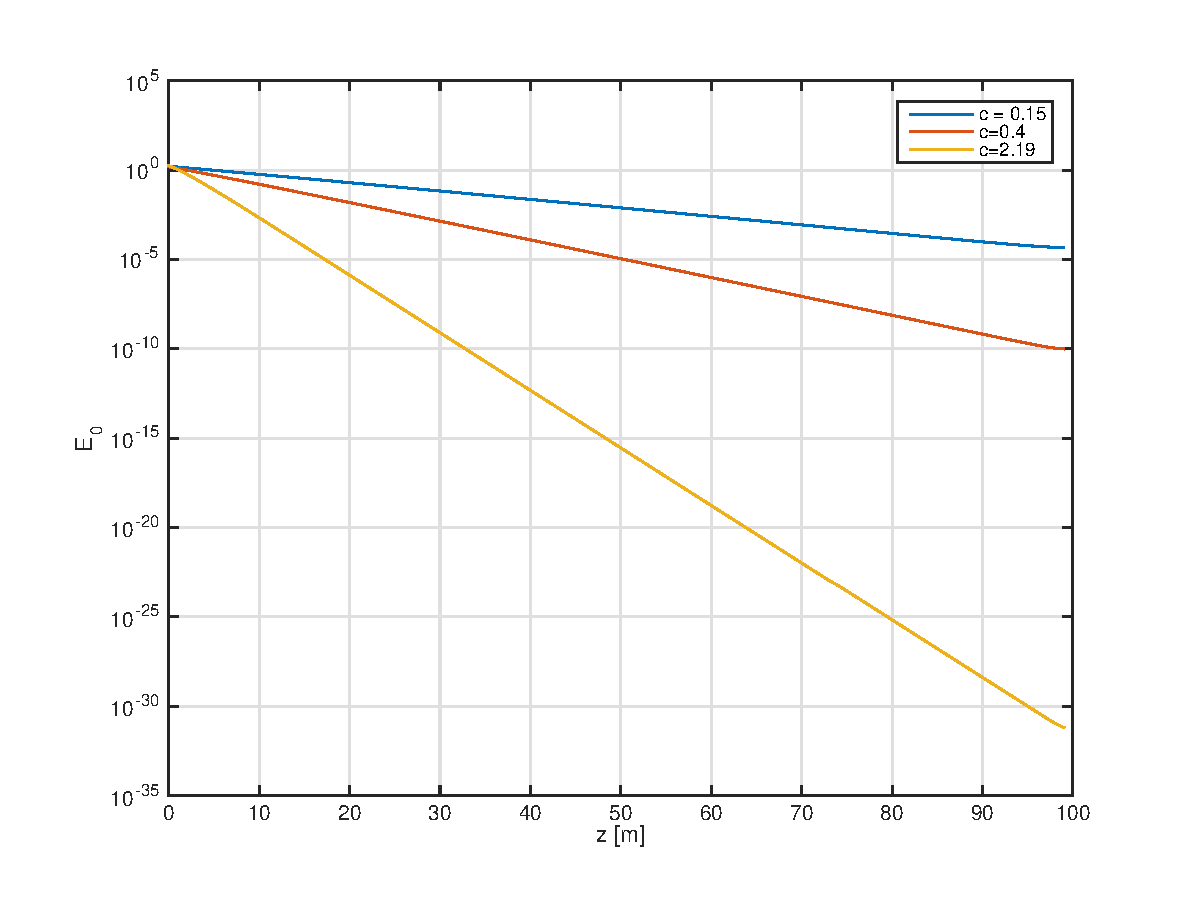
\includegraphics[width = 0.7\textwidth]{e0_z}
	\caption{Irradiance $E_0$ vs. $z$}
	\label{fig:e0zm}
\end{figure}

Some evaluation on the propagation are then carried out with a MATLAB script that uses the provided parameters for receiver and transmitter. The propagation model used the one proposed in~\cite{optmodel} and assumes that there is a successful transmission if the SNR is over a certain threshold. In particular from the irradiance and the parameters $S$ (sensitivity) and $A_r$ (area of the receiver) of the considered modem it is possible to compute the power of ambient light noise, which is $N_A = (S E_0 A_r)^2$. Let the received power $P$ be
\begin{equation}
	P = \frac{2 P_{tx} A_r \cos(\beta)}{\pi d^2 (1-\cos(\theta)) + 2 A_t}e^{-cd}
	\label{eq:p_opt}
\end{equation}
then the SNR is
\begin{equation}
	\Gamma  = \frac{(SP)^2}{2q(I_D + I_L)BW + \frac{4KTBW}{R} + N_A}
	\label{eq:snr_opt}
\end{equation}
In the following, if the SNR is above the threshold of 20 dB then there is a successful transmission. In particular, by setting the threshold and a distance $d = 10$ m, by inverting~\eqref{eq:snr_opt} in order to get $P$ and~\eqref{eq:p_opt} in order to compute $P_{tx}$ it is possible to know which is the minimum transmission power that can be used to reach a distance $d$. In Figure~\ref{fig:ptx}[a] there is the plot of the minimum $P_{tx}$ against the irradiance $E_0$, while in Figure~\ref{fig:ptx}[b] the x axis is the depth $z$ considered.

\begin{figure}[h!]
	\centering
	\subfigure[$P_{tx}$ to reach $d = 10$ m as a function of $E_0$]{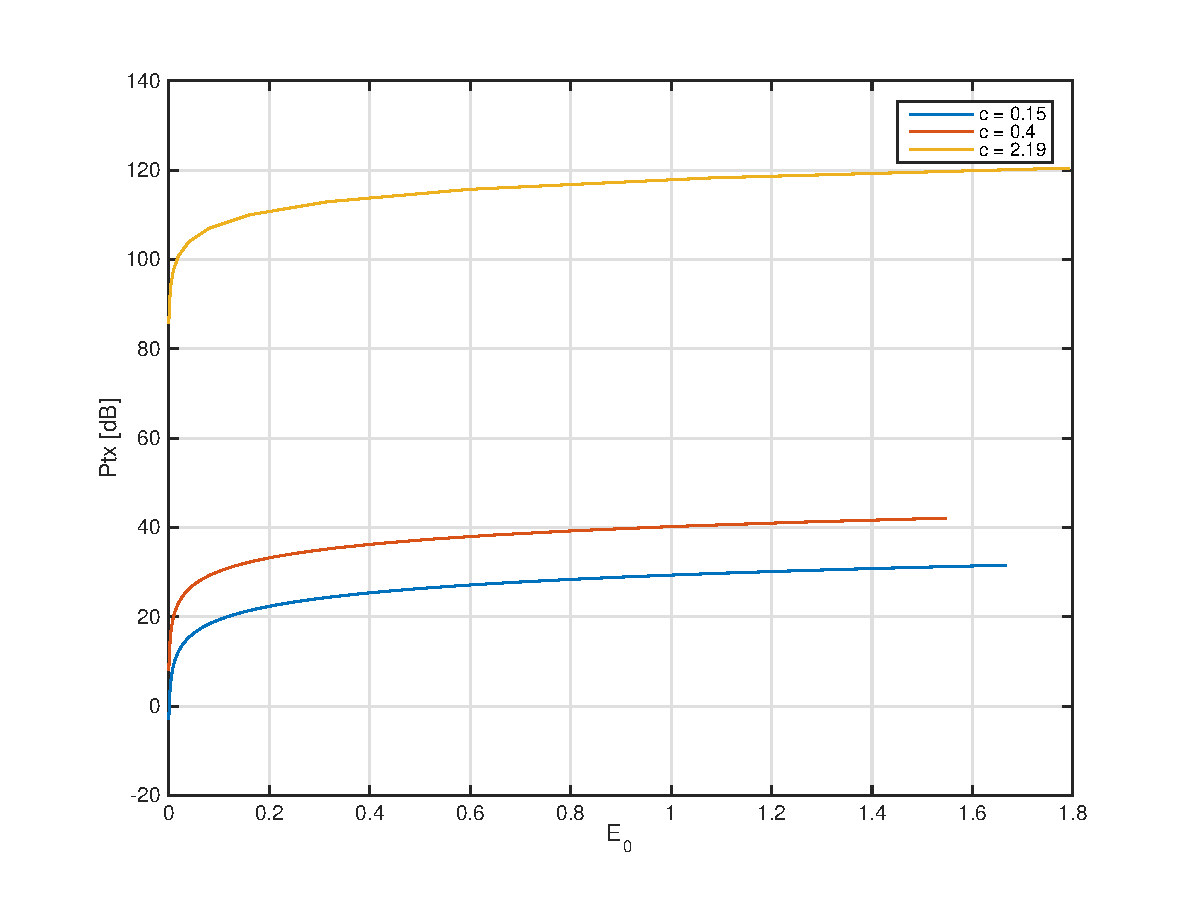
\includegraphics[width = 0.45\textwidth]{ptx_e0}}
	\subfigure[$P_{tx}$ to reach $d = 10$ m as a function of $z$]{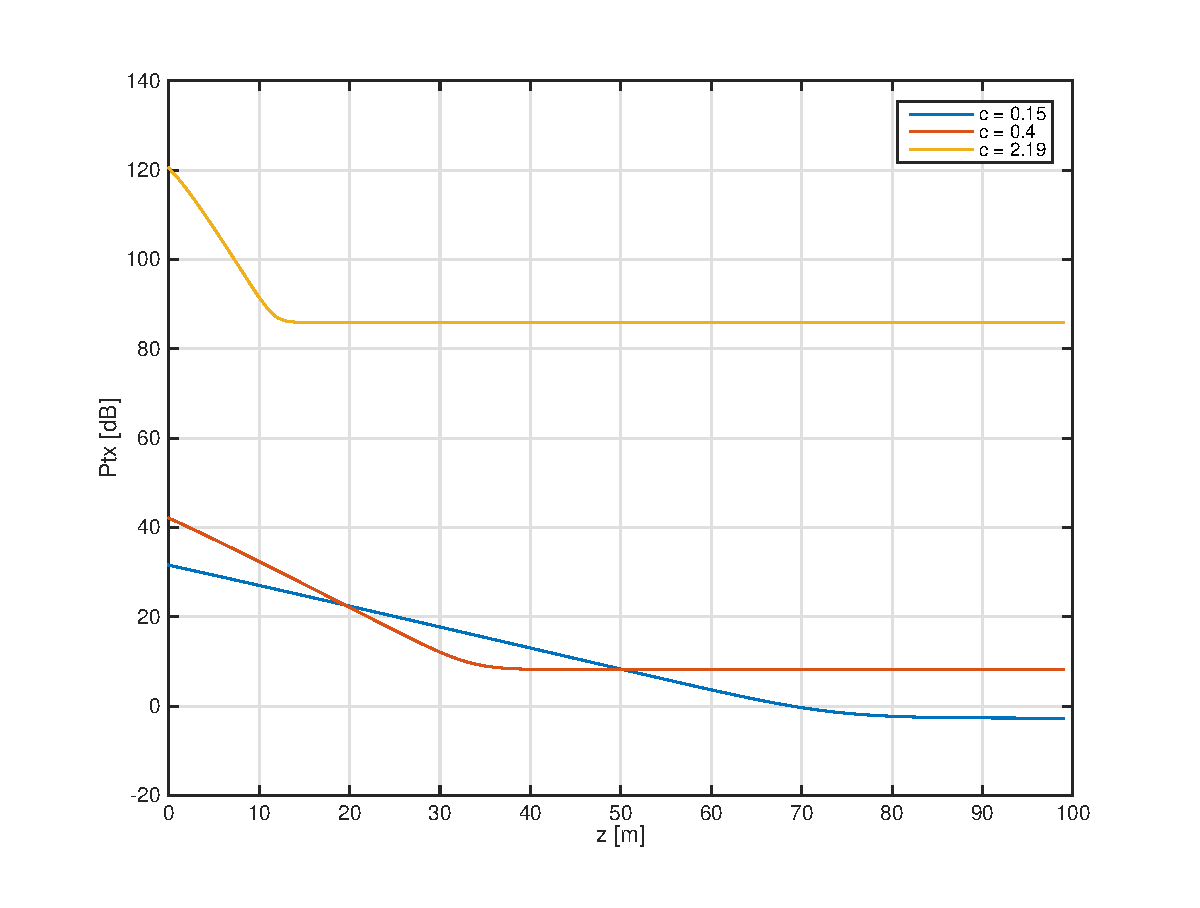
\includegraphics[width = 0.45\textwidth]{ptx_z}}
	\caption{Transmitted power $P_{tx}$ required to transmit at a distance of $d = 10$ meters}
	\label{fig:ptx}
\end{figure}

Finally, the transmit power is set to $P_{tx, max} = 100$ W and the maximum distance at which is possible to transmit is evaluated. Note that~\eqref{eq:p_opt} is not invertible with respect to the distance $d$, therefore the received power $P$ given by~\eqref{eq:p_opt} is precomputed for $d \in [0, 50]$ m and stored in a vector \texttt{P\_d}. Then, given a certain $E_0$, from~\eqref{eq:snr_opt} the minimum received power to guarantee an SNR of 20 dB is computed and the closest $P$ in \texttt{P\_d} is found. The corresponding value of $d$ is chosen as the maximum distance $d_{max}$ at which it is possible to transmit with $P_{tx, max} = 100$ W and that $E_0$ - or the corresponding $z$.

The results are in Figure~\ref{fig:dmax}.

\begin{figure}[h!]
	\centering
	\subfigure[$d_{max}$ as a function of $E_0$, for $P_{tx, max} = 100$]{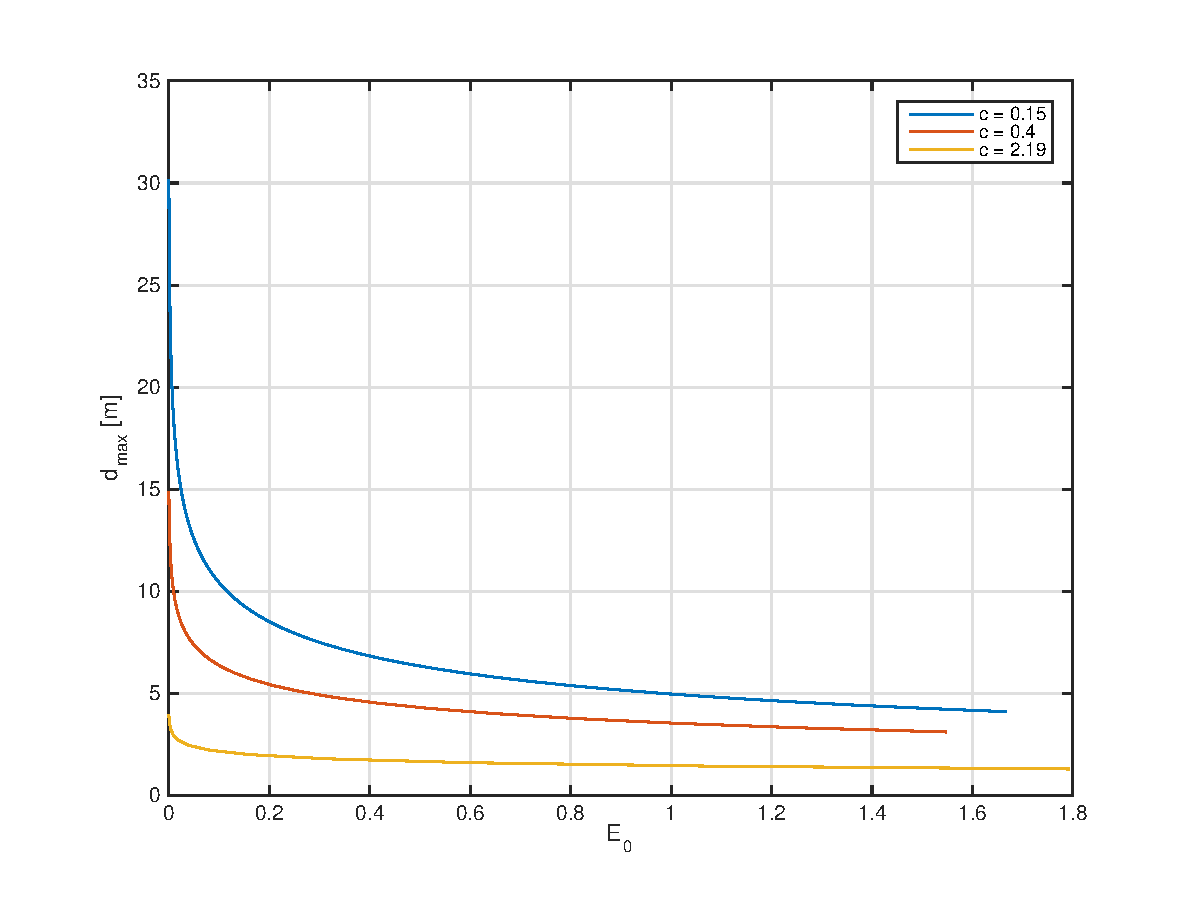
\includegraphics[width= 0.45\textwidth]{dmax_e0}}
	\subfigure[$d_{max}$ as a function of $z$, for $P_{tx, max} = 100$]{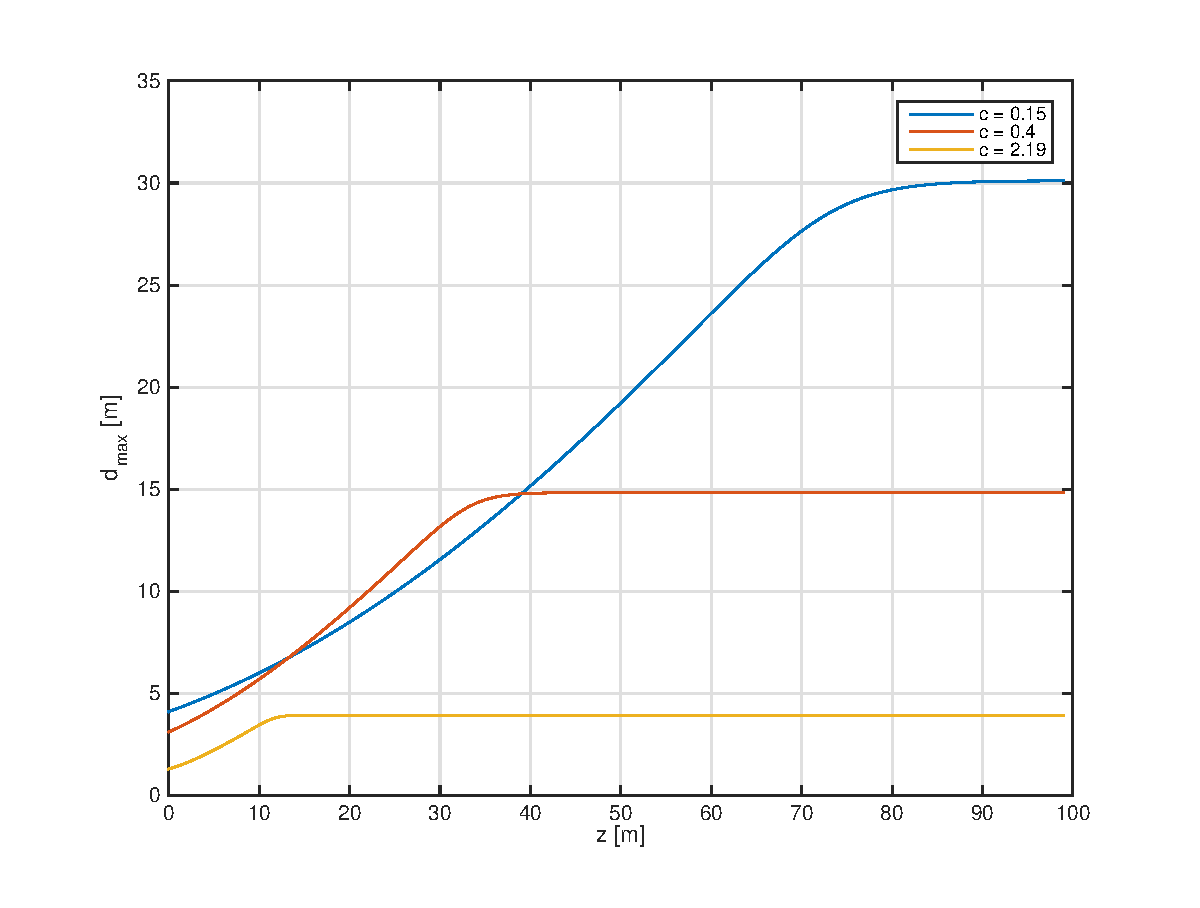
\includegraphics[width= 0.45\textwidth]{dmax_z}}
	\caption{Maximum distance $d_{max}$ with a transmit power of $P_{tx, max} = 100$}
	\label{fig:dmax}
\end{figure}


\begin{thebibliography}{10}

\bibitem{leb}
Y. Le Boudec, Performance Evaluation of Computer and Communications Systems, EPFL, 2015

\bibitem{optmodel}
D. Anguita et al., Optical wireless underwater communication for AUV: Preliminary simulation and experimental results, in Proc. IEEE/OES Oceans, Santander, Spain, Jun. 2011

\end{thebibliography}

\end{document}
